
\begin{figure}[!ht]
  \centering
  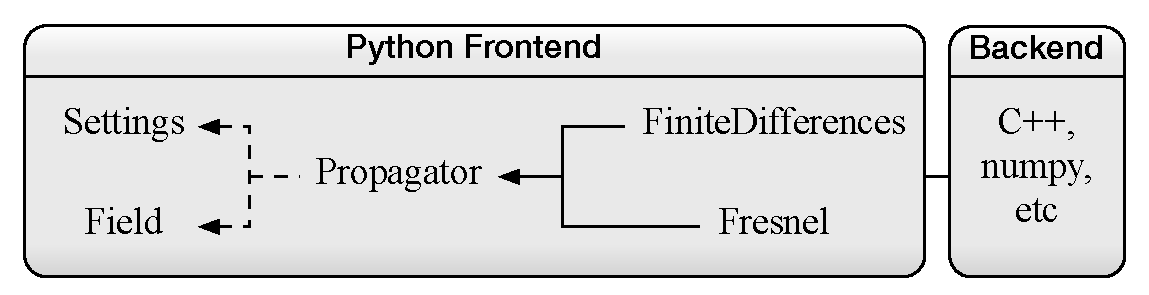
\includegraphics[width=0.8\textwidth]{implementation/frontend.pdf}
  \caption{Frontend/backend overview and a simplified class diagram for the propagator object. Solid lines represent inheritance while dashed lines represent usage.}
  \label{fig:program_structure}
\end{figure}


\subsection{Frontend}

Our goal was to create a fast implementation of the propagation algorithms while keeping the front-end as easy to use and general as possible. We chose python 2.7~\cite{python} as the front-end scripting language as it is widely accepted in the scientific community, has a broad ecosystem of third-party libraries and is free and open-source. Another goal was a clean separation of physical properties of the simulated system (e.g. $k$, $n(x,y,z)$, etc.) and numerical details (e.g. $N_x$, $\Delta x$, propagators, etc.) in the user interface. We solved this by developing the symbolic term-rewriting engine \emph{Expresso}~\cite{lars_melchior_2016_46539} which allows us to design an arbitrary level of abstraction in the end-interface.

Simulation parameters are stored as term-rewriting rules in a \lstinline{Settings} object as and can be interdependent. They are then evaluated or compiled to Python-Numpy or C++~\cite{standard_c++} code at any abstraction level when necessary. Propagators are initialized with such a \lstinline{Settings} object and create the initial field $u_{i,j}^0$. They implement a \lstinline{step()} function that updates the field from $u_{i,j}^k$ to $u_{i,j}^{k+1}$.

\subsection{Fresnel Propagator \label{sec:fresnel_propagator_implementation}}

Depending on the value of $F$ the Fresnel propagator will perform a different step scheme. With $R := \frac{1}{2 \pi} \exp \! \left( F \Delta z \right)$ and $D := \exp( - A \Delta z (k_x^2+k_y^2) )$

\begin{itemize}
    \item $F = c \in \mathbb{C}$: The initial field is Fourier transformed once and multiplied element-wise with $R \cdot D$ in each step. The reverse transform is only performed to retrieve the field.
    \item $F = F(x,y,z)$: In each step the current field is Fourier transformed, multiplied element-wise with $D$, transformed back and multiplied element-wise with $R$ (multi-slice approach).
\end{itemize}

If the python library \lstinline{pyFFTW} is installed on the host computer the Fourier transforms are optimized for the current hardware and evaluated in parallel. Otherwise the \lstinline{numpy} FFT methods are used.  

\subsection{Finite Difference Propagator}

\subsubsection{Tridiagonal matrix inversion}

Using Thomas' Algorithm~\cite{Press:1992:NRC:148286}, which is a simplified form of Gaussian elimination, the matrix equations \eqref{eq:FD1DMatrixEquation} and \eqref{eq:FD2DMatrixEquation} can be solved very efficiently. This algorithm has been shown to be stable in many cases, particularly when the matrix involved is diagonally dominant~\cite{Press:1992:NRC:148286}. We show that the tridiagonal matrix $B$ in equation \eqref{eq:FD1DMatrixEquation} is diagonally dominant if $|C_i^k| \le 1$. For all $i \in \{1..n_x\}$ and $k \in \{1..n_z\}$:

\begin{align*}
    |B_{ii}^k| \ge \sum_{j \ne i} |B_{ij}^k| & \Leftrightarrow |1 + 2r_x - C_i^k|\ge \left|1 + 2r_x - |C_i^k| \right| \ge 2 r_x \\
    & \Rightarrow |C_i^k| \le 1 \; \vee \; |C_i^k| \ge 1 + 4 r_x .
\end{align*}

This can be done analogously for equation \eqref{eq:FD2DMatrixEquation}. For $n \ne 1$, this gives us a condition for the step size $\Delta z$ that ensures numerical stability:

\begin{align*}
    \frac{\Delta z}{\lambda} \le \frac{2}{\pi} \frac{1}{\max |n^2 - 1|},
\end{align*}

where the maximum must be taken over all points inside the simulation box. If $n = 1$ everywhere any step size is numerically stable and $\Delta z$ can be chosen according to the desired numerical accuracy.

\subsubsection{Parallel implementation}

The equations in the equation system \eqref{eq:FD2DMatrixEquation} do not depend on each other and can therefore be solved in parallel. Work is hereby divided nearly evenly among all cores of the computer. Typical simulation times on a 2011 consumer notebook are seconds for a 2D simulation or minutes for a 3D simulation.


